Alternative data visualization techniques can be found using the power of barycentric coordinates and GPU programming.

The usual way to visualize data for a triangle mesh is to associate data to vertices and then interpolating over the mesh triangles, that does not work in case of edges and triangles.

\section{Region around a vertex}
We can split the surface of triangle meshes into regions around vertex (Fig. \ref{fig:vertex-area}) and color them.

These regions can be determined using barycentric coordinates and GPU fragment program. Visualizing data given at the vertices or edges of the mesh in a piecewise constant simulates the classical triangle flat shading.
An example of this vertex data is the discrete Gaussian curvature.
\begin{figure}[h]
    \centering
    \minipage[b]{.5\linewidth}
    \centering
    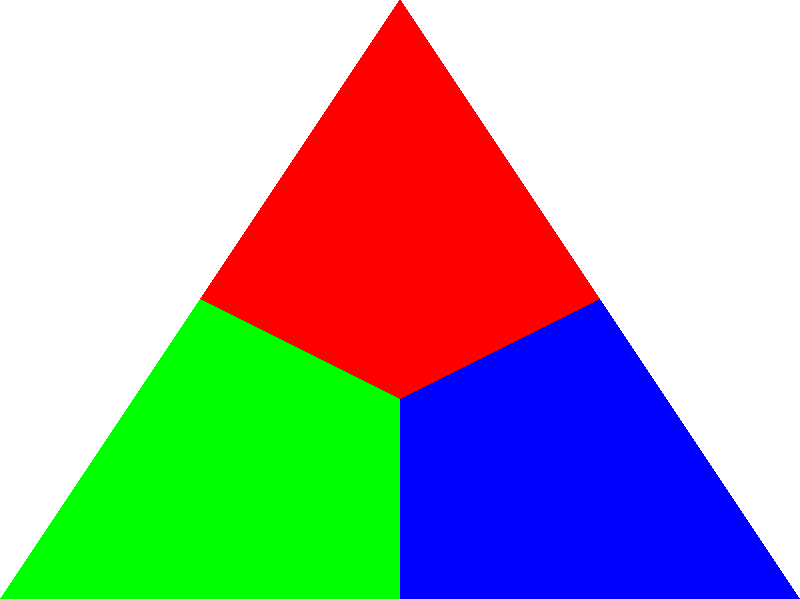
\includegraphics[scale=0.2]{images/max.png}
    \caption{Vertex based area}\label{fig:max-diagram}
    \endminipage
    \minipage[b]{.5\linewidth}
    \centering
    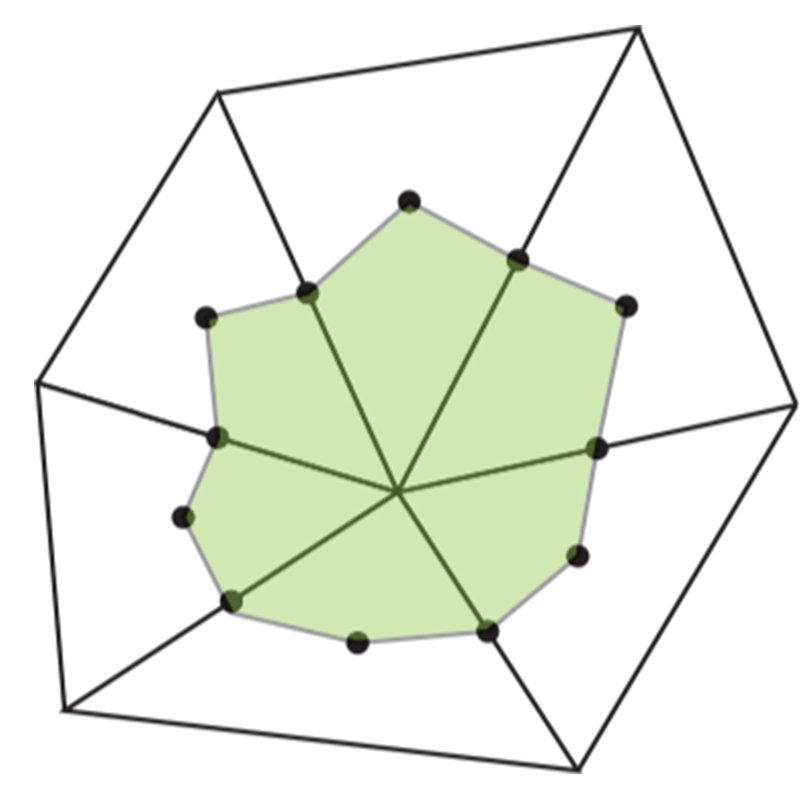
\includegraphics[scale=0.2]{images/vertex-area.png}
    \caption{Region around a vertex}\label{fig:vertex-area}
    \endminipage
\end{figure}


\section{Max diagram - Vertex based area}
Passing barycentric coordinates to the fragment shader will clearly demonstrate that we can get results different from the classic color interpolation.

There are different approaches to color interpolation focusing on the distance from vertices. For each point in a triangle, we can easily determine its closest vertex, which we use as a cue for coloring.

A different approach from interpolating, can be found coloring vertex areas based on the minimum barycentric coordinate.
The color is given by the region farthest from a vertex (Fig. \ref{fig:max-diagram}).

\begin{lstlisting}[language=C++,
    directivestyle={\color{black}}
    emph={int,char,double,float,unsigned},
    emphstyle={\color{blue}}
   ]
if (Coords.x > Coords.y && Coords.x > Coords.z) {
    vec3 blue = vec3(0.0f, 0.0f, 1.0f);
    FragColor = vec4(blue, 1.0f);
} else if(Coords.y > Coords.x && Coords.y > Coords.z) {
    vec3 green = vec3(0.0f, 1.0f, 0.0f);
    FragColor = vec4(green, 1.0f);
} else {
    vec3 red = vec3(1.0f, 0.0f, 0.0f);
    FragColor = vec4(red, 1.0f);
}
\end{lstlisting}

\section{Implementation}
Suppose now that you want each vertex area to be in one constant color. This color can be taken from shading interpolation using the normal at the vertex and the vertex position. Then you can compute the color has it be done in \textit{Gouraud Shading}.

The idea is to compute the color per vertex but instead of linearly interpolated it in each triangle (as \textit{Gouraud shading} does) we color regions around a vertex with that constant color.

To implement that we need to pass the barycentric coordinates, the vertex color, the normal at the vertex and the lighting calculations to the \textit{fragment shader}.

We want to avoid an automatic interpolation of colors, in order to return the resulting color using the \textit{max diagram}, to do that we have used a \textit{Geometry shader} in order to access to all three vertex colors in fragment shader.
\\
\\
\scalebox{0.85}{\begin{tikzpicture}
    [node distance=.8cm,
    start chain=going right,]
       \node[punktchain, join] (vs) {Vertex Shader};
       \node[punktchain, join] (gs)  {Geometry Shader};
       \node[punktchain, join] (fs)  {Fragment Shader};
\end{tikzpicture}}
